%Este trabalho está licenciado sob a Licença Atribuição-CompartilhaIgual 4.0 Internacional Creative Commons. Para visualizar uma cópia desta licença, visite http://creativecommons.org/licenses/by-sa/4.0/deed.pt_BR ou mande uma carta para Creative Commons, PO Box 1866, Mountain View, CA 94042, USA.

\chapter{Produto vetorial}\label{cap_prodvet}
\thispagestyle{fancy}

De agora em diante, vamos trabalhar com um base ortonormal $B = (\vec{i}, \vec{j}, \vec{k})$ dita com orientação positiva, i.e. os vetores $\vec{i} = \overrightarrow{OI}$, $\vec{j} = \overrightarrow{OJ}$ e $\vec{k}=\overrightarrow{OK}$ estão dispostos em sentido anti-horário, veja Figura \ref{fig:base_pos}.

\begin{figure}[H]
  \centering
  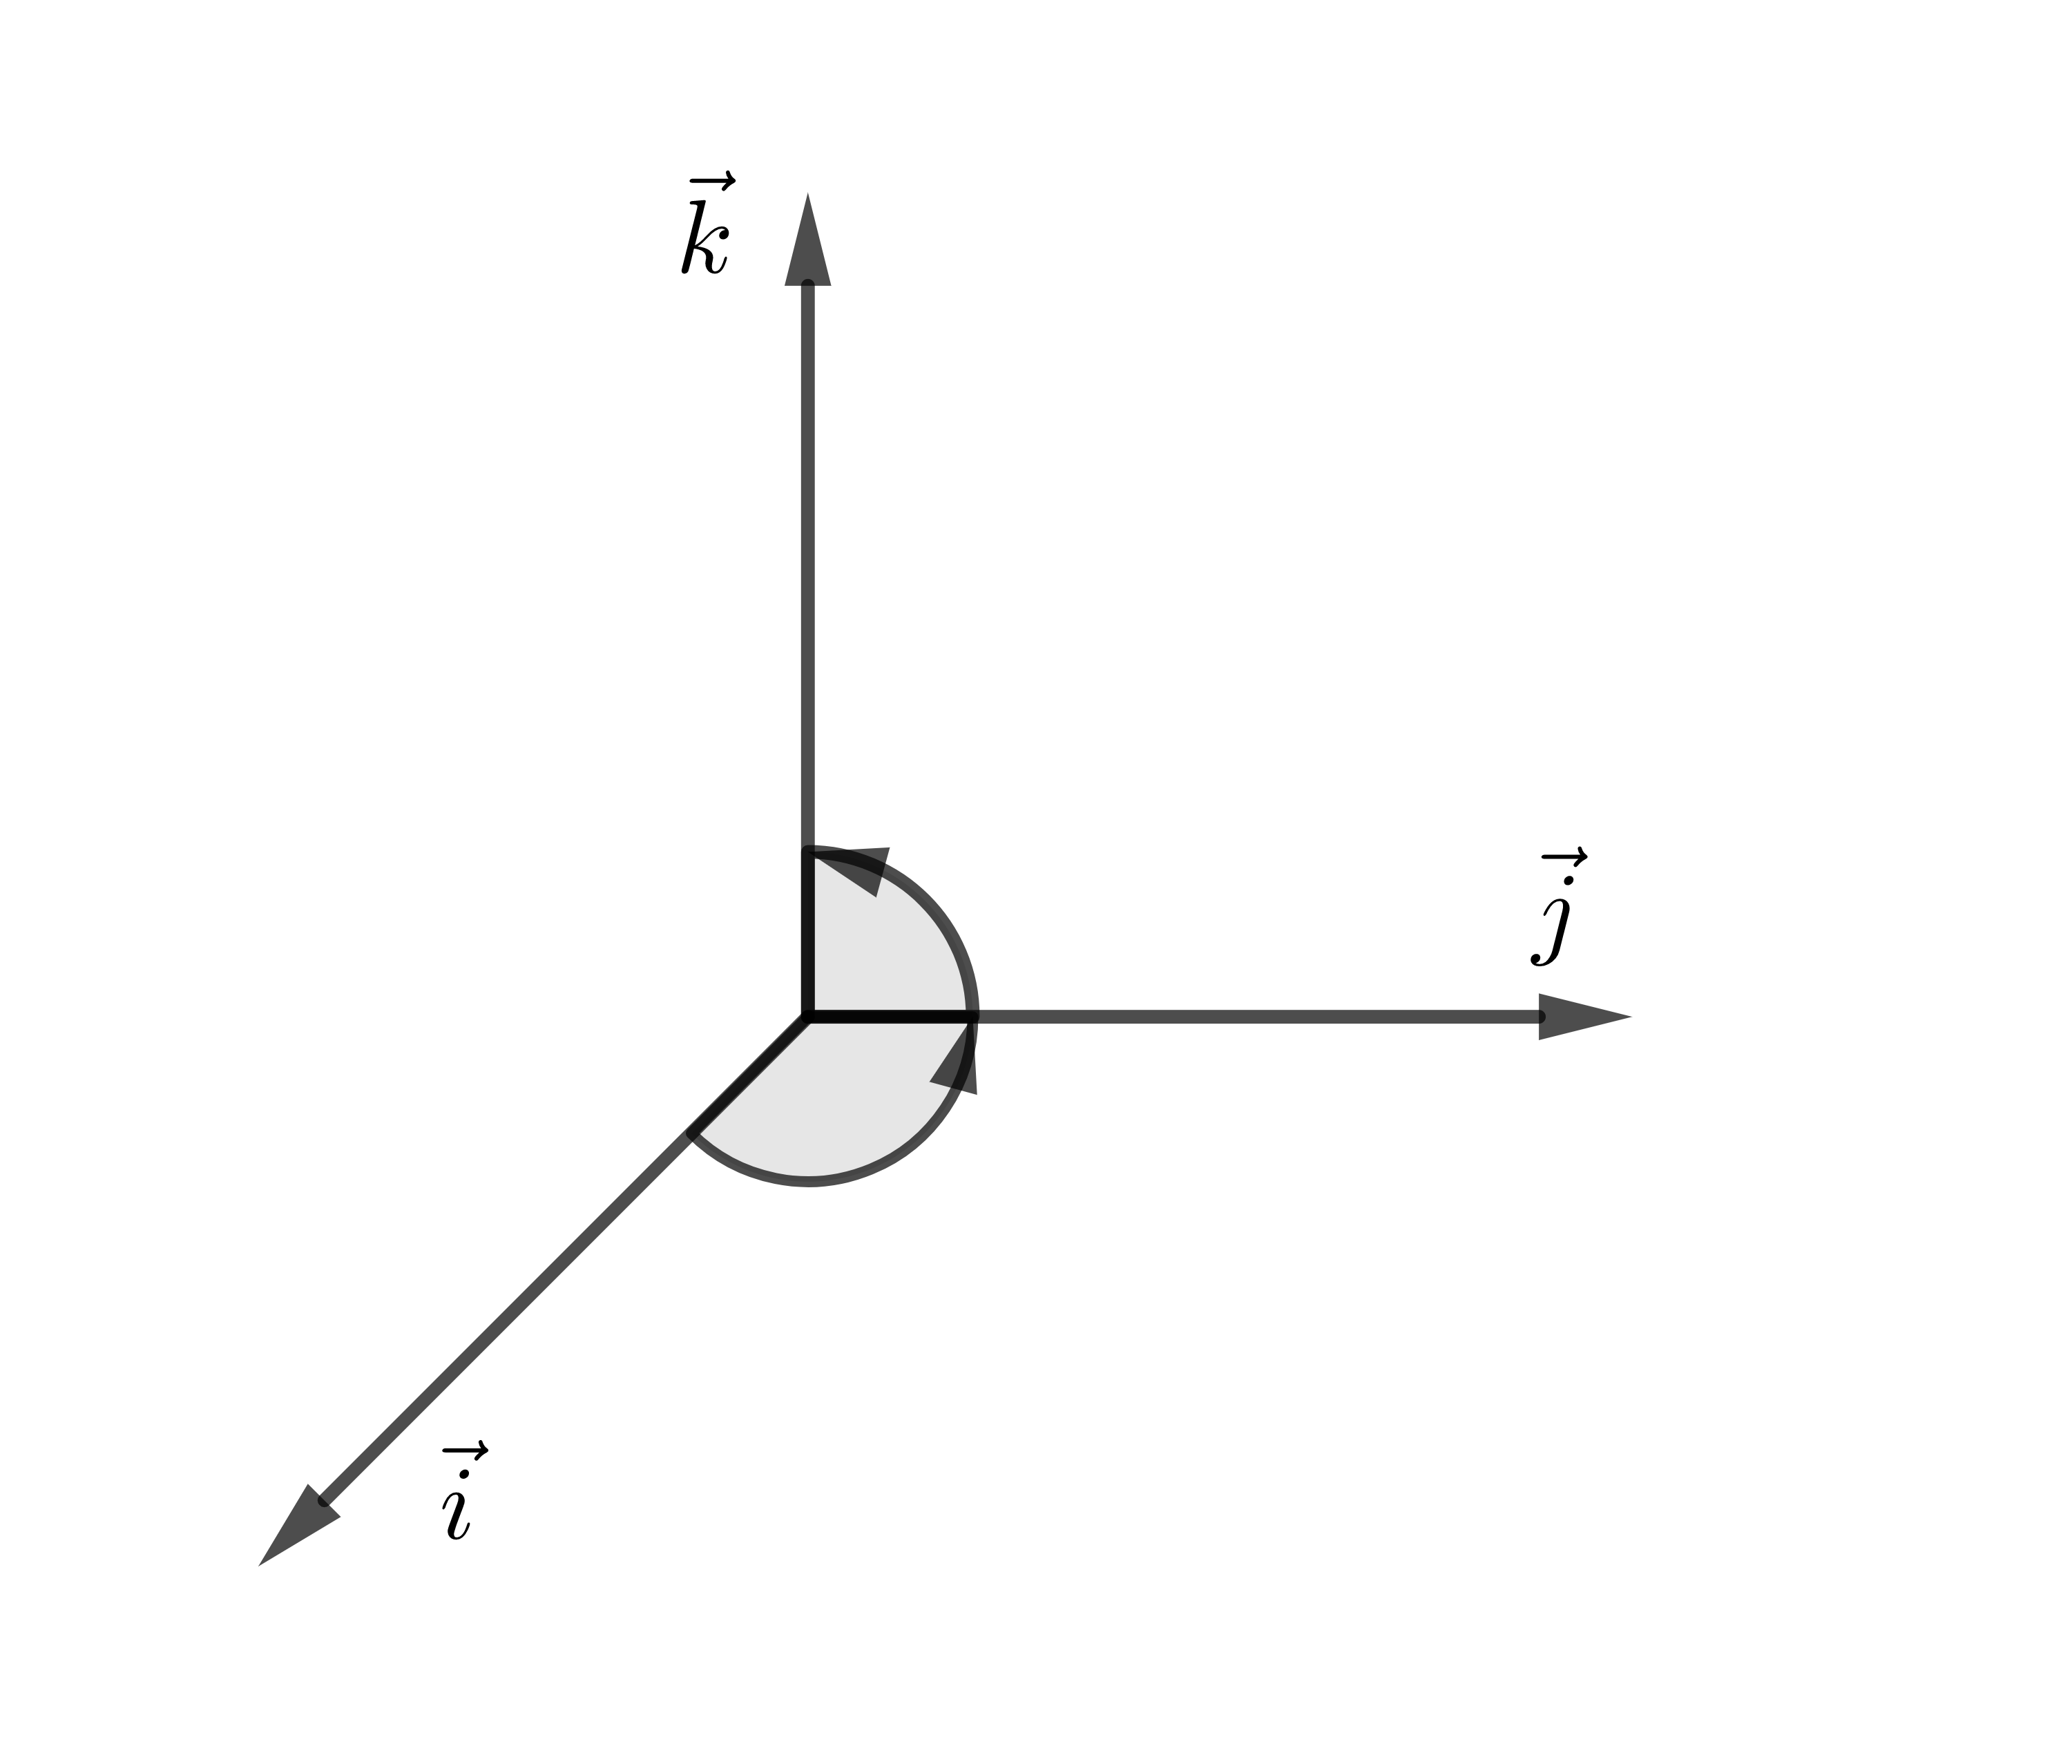
\includegraphics[width=0.7\textwidth]{./cap_prodvet/dados/fig_base_pos/fig_base_pos}
  \caption{Base ortonormal positiva.}
  \label{fig:base_pos}
\end{figure}

\section{Definição}\label{cap_prodvet_sec_prodvet}

Dados vetores $\vec{u}$ e $\vec{v}$, definimos o produto vetorial de $\vec{u}$ com $\vec{v}$, denotado por $\vec{u}\land\vec{v}$, como o vetor:
\begin{itemize}
\item se $\vec{u}$ e $\vec{v}$ são l.d., então $\vec{u}\land\vec{v} = \vec{0}$.
\item se $\vec{u}$ e $\vec{v}$ são l.i., então
  \begin{itemize}
  \item $|\vec{u}\land\vec{v}| = |\vec{u}||\vec{v}|\sen\alpha$, onde $\alpha$ é o ângulo entre $\vec{u}$ e $\vec{v}$,
  \item $\vec{u}\land\vec{v}$ é ortogonal a $\vec{u}$ e $\vec{v}$, e
  \item $\vec{u}$, $\vec{v}$ e $\vec{u}\land\vec{v}$ formam uma base positiva.
  \end{itemize}
\end{itemize}

\subsection{Interpretação geométrica}

Sejam dados $\vec{u}$ e $\vec{v}$ l.i.. Estes vetores determinam um paralelogramo, veja Figura \ref{fig:prodvet_interp}. Seja, então, $h$ a altura deste paralelogramo tendo $\vec{u}$ como sua base. Logo, a área do paralelogramo é o produto do comprimento da base com sua altura, neste caso
\begin{equation}
  |\vec{u}|h = |\vec{u}||\vec{v}|\sen\alpha.
\end{equation}
Ou seja, o produto vetorial $\vec{u}\land\vec{v}$ tem norma igual à área do paralelogramo determinado por $\vec{u}$ e $\vec{v}$.

\begin{figure}[H]
  \centering
  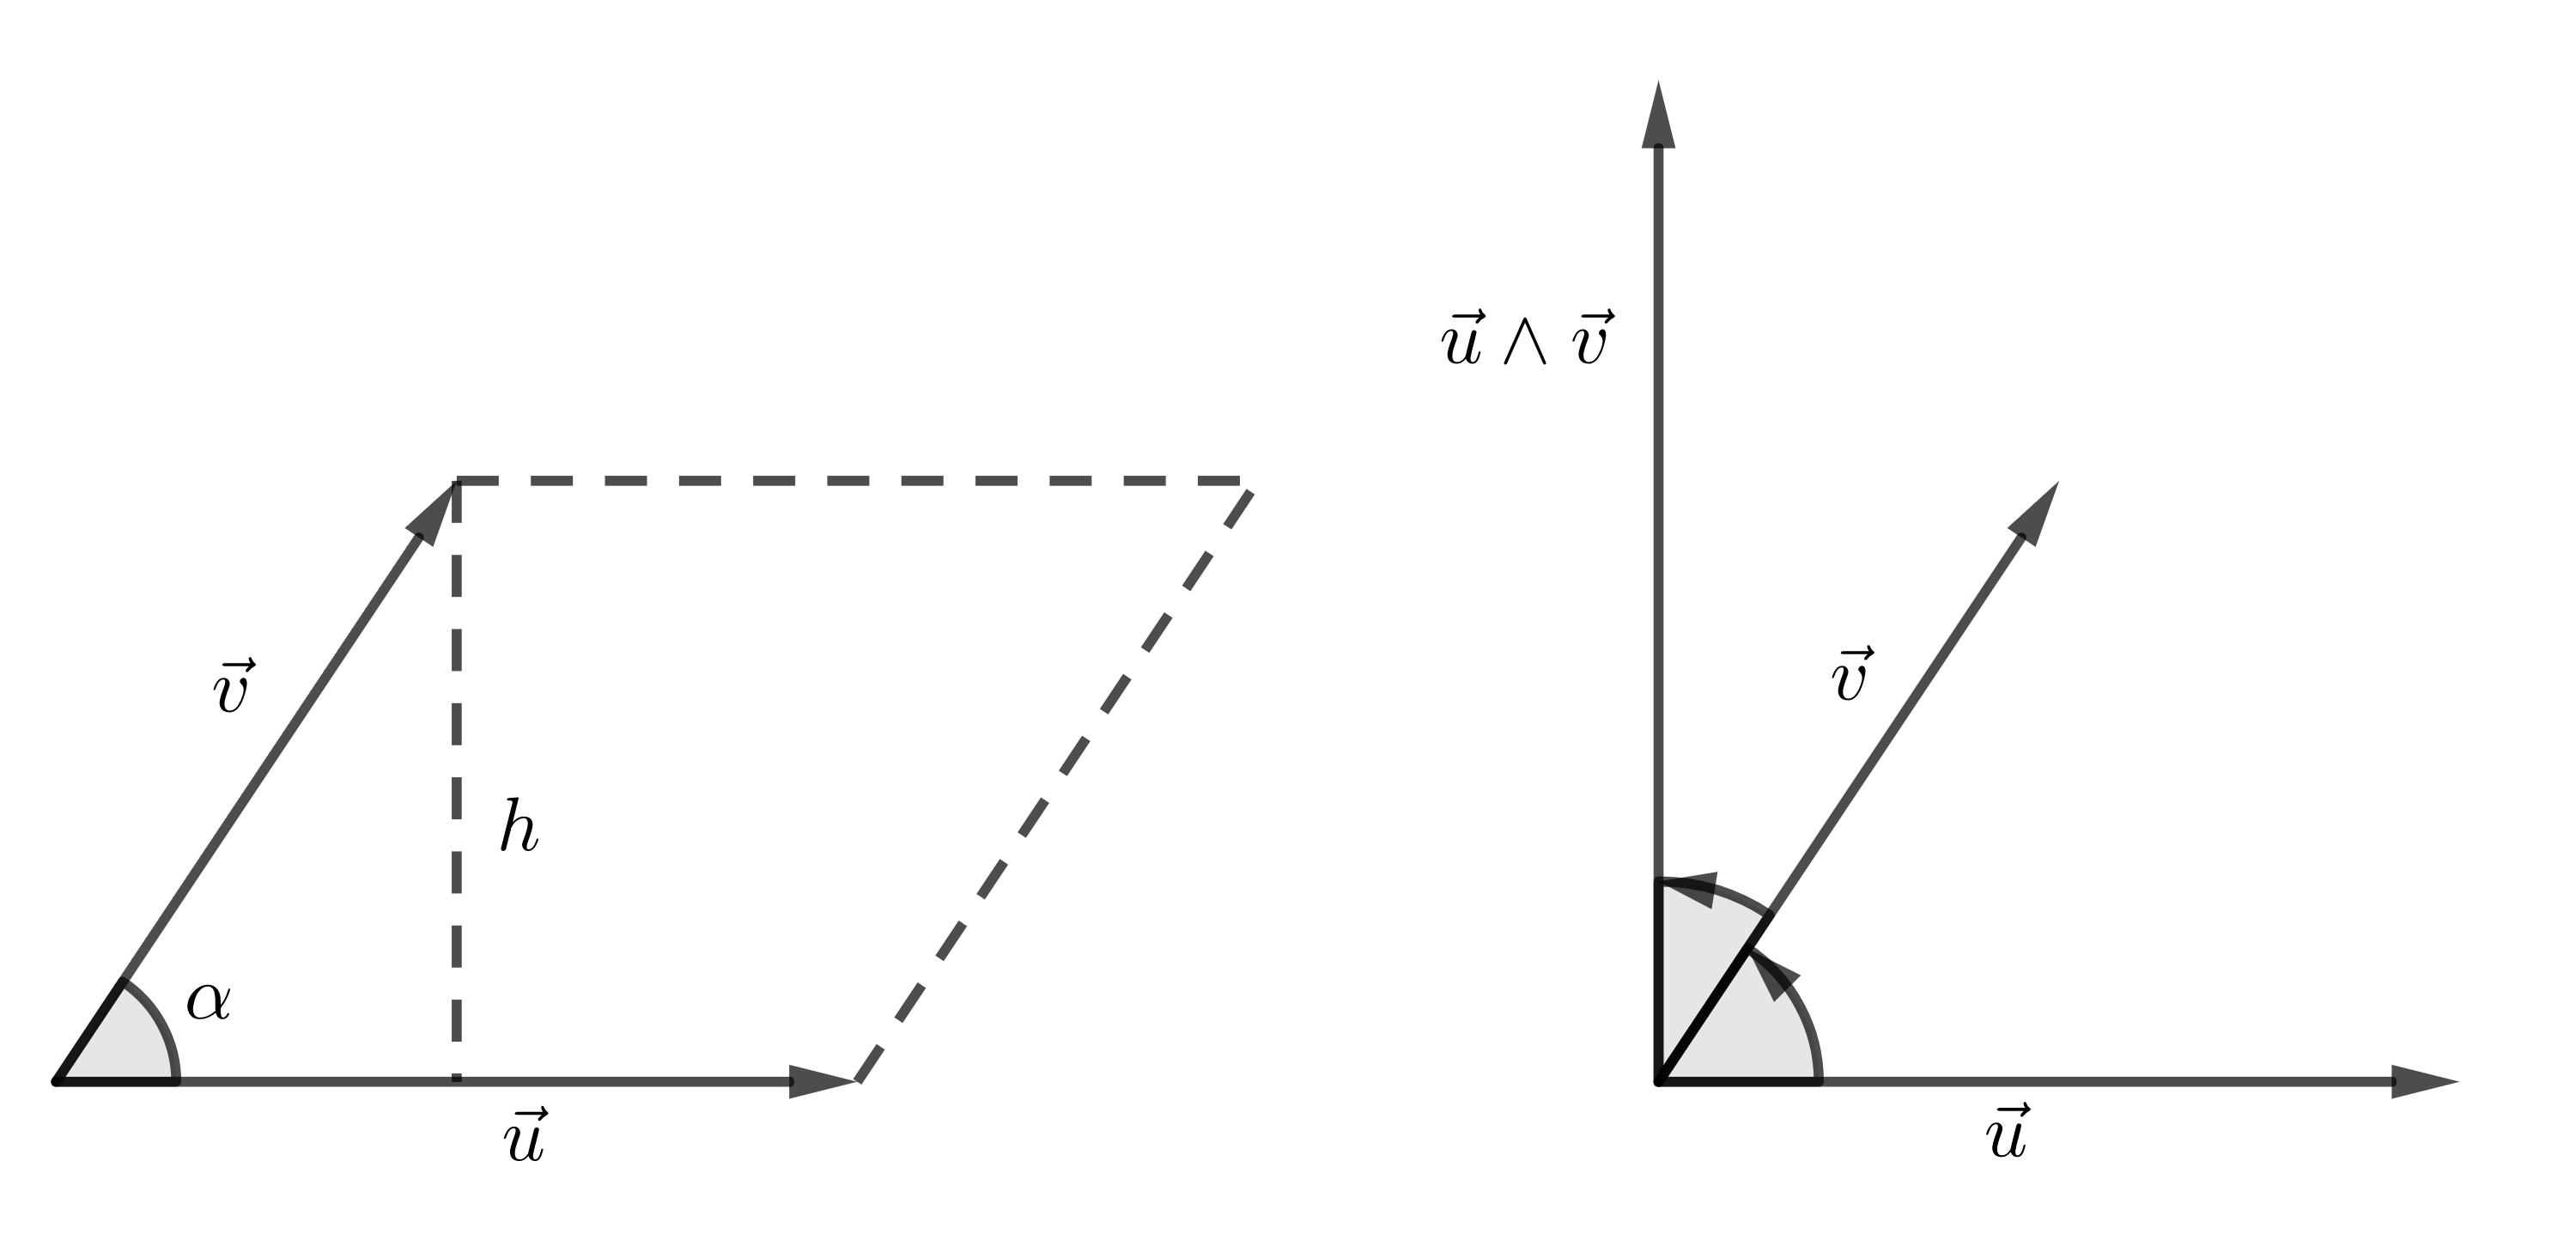
\includegraphics[width=0.7\textwidth]{./cap_prodvet/dados/fig_prodvet_interp/fig_prodvet_interp}
  \caption{Base ortonormal positiva.}
  \label{fig:base_pos}
\end{figure}

\subsection{Produto vetorial via coordenadas}\label{cap_prodvet_sec_coord}

Dados $\vec{u} = (u_1,u_2,u_3)$ e $\vec{v} = (v_1,v_2,v_3)$ em uma base ortonormal positiva, então
\begin{equation}
  \vec{u}\land\vec{v} =
  \begin{vmatrix}
    u_2 & u_3\\
    v_2 & v_3
  \end{vmatrix}\vec{i} -
  \begin{vmatrix}
    u_1 & u_3\\
    v_1 & v_3
  \end{vmatrix}\vec{j} +
  \begin{vmatrix}
    u_1 & u_2 \\
    v_1 & v_2
  \end{vmatrix}\vec{k}.
\end{equation}

\begin{obs}
  Uma regra mnemônica, é
  \begin{equation}
    \vec{u}\land\vec{v} =
    \begin{vmatrix}
      \vec{i} & \vec{j} & \vec{k} \\
      u_1 & u_2 & u_3 \\
      v_1 & v_2 & v_3
    \end{vmatrix}.
  \end{equation}
\end{obs}

\begin{ex}
  Dados os vetores $\vec{u} = (1,-2,1)$ e $\vec{v} = (0,2,-1)$, temos
  \begin{align}
    \vec{u}\land\vec{v} &=
                          \begin{vmatrix}
                            \vec{i} & \vec{j} & \vec{k} \\
                            u_1 & u_2 & u_3 \\
                            v_1 & v_2 & v_3
                          \end{vmatrix} \\
                        &=
                          \begin{vmatrix}
                            \vec{i} & \vec{j} & \vec{k} \\
                            1       & -2      & 1 \\
                            0       & 2       & -1
                          \end{vmatrix} \\
                        &= 0\vec{i} + \vec{j} + 2\vec{k}\\
                        &= (0,1,2).
  \end{align}
\end{ex}

\subsection{Exercícios}

\emconstrucao

\section{Propriedades do produto vetorial}\label{cap_prodvet_sec_prop}

Nesta seção, discutiremos sobre algumas propriedades do produto vetorial. Para tanto, sejam dados os vetores $\vec{u} = (u_1,u_2,u_3)$, $\vec{v}=(v_1,v_2,v_3)$, $\vec{w}=(w_1,w_2,w_3)$ e o número real $\gamma$.

Da definição do produto vetorial, temos $\vec{u}\perp(\vec{u}\land\vec{v})$ e $\vec{v}\perp(\vec{u}\land\vec{v})$, logo
\begin{equation}
  \vec{u}\cdot(\vec{u}\land\vec{v}) = 0\quad\text{e}\quad\vec{v}\cdot(\vec{u}\land\vec{v}) = 0.
\end{equation}

Em relação à multiplicação por escalar, temos
\begin{equation}
  \gamma(\vec{u}\land\vec{v}) = (\gamma\vec{u})\land\vec{v} = \vec{u}\land(\gamma\vec{v}).
\end{equation}
De fato,
\begin{align}
  (\gamma\vec{u}\land\vec{v}) &=
                                \begin{vmatrix}
                                  \vec{i} & \vec{j} & \vec{k} \\
                                  \gamma u_1 & \gamma u_2 & \gamma u_3\\
                                  v_1 & v_2 & v_3
                                \end{vmatrix} \\
                              &=
                                \begin{vmatrix}
                                  \vec{i} & \vec{j} & \vec{k} \\
                                  u_1 & u_2 & u_3\\
                                  \gamma v_1 & \gamma v_2 & \gamma v_3
                                \end{vmatrix} = \vec{u}\land(\gamma\vec{v})\\
                              &= \gamma\begin{vmatrix}
                                  \vec{i} & \vec{j} & \vec{k} \\
                                  u_1 & u_2 & u_3\\
                                  v_1 & v_2 & v_3
                                \end{vmatrix} = \gamma(\vec{u}\land\vec{v}).\\
\end{align}

Também, vale a propriedade distributiva com a operação de soma, i.e.
\begin{equation}
  \vec{u}\land(\vec{v} + \vec{w}) = \vec{u}\land\vec{v}+\vec{u}\land\vec{w}.
\end{equation}
De fato, temos
\begin{align}
  \vec{u}\land(\vec{v}+\vec{w}) &=
                                  \begin{vmatrix}
                                    \vec{i} & \vec{j} & \vec{k} \\
                                    u_1 & u_2 & u_3 \\
                                    v_1+w_1 & v_2+w_2 & u_3+w_3
                                  \end{vmatrix} \\
                                &=
                                  \begin{vmatrix}
                                    \vec{i} & \vec{j} & \vec{k} \\
                                    u_1 & u_2 & u_3 \\
                                    v_1 & v_2 & v_3                                    
                                  \end{vmatrix}
                                                +
                                                \begin{vmatrix}
                                                  \vec{i} & \vec{j} & \vec{k} \\
                                                  u_1 & u_2 & u_3 \\
                                                  w_1 & w_2 & w_3                                    
                                                \end{vmatrix}\\
                                &= \vec{u}\land\vec{v} + \vec{u}\land\vec{w}.
\end{align}

Observamos que o produto vetorial não é comutativo, entretanto
\begin{equation}
  \vec{u}\land\vec{v} = -\vec{v}\land\vec{u}.
\end{equation}
De fato, temos
\begin{align}
  \vec{u}\land\vec{v} &= \begin{vmatrix}
                         \vec{i} & \vec{j} & \vec{k} \\
                         u_1 & u_2 & u_3 \\
                         v_1 & v_2 & v_3                                    
                       \end{vmatrix}\\
                      &= -\begin{vmatrix}
                         \vec{i} & \vec{j} & \vec{k} \\
                         v_1 & v_2 & v_3 \\
                         u_1 & u_2 & u_3                                    
                       \end{vmatrix}\\
                      &= -\vec{v}\land\vec{u}.
\end{align}

Também, o produto vetorial não é associativo sendo $(\vec{u}\land\vec{v})\land\vec{w}$, em geral, diferente de $\vec{u}\land(\vec{v}\land\vec{w})$. Com efeito, temos
\begin{align}
  (\vec{i}\land\vec{i})\land\vec{j} &= \vec{0},\\
  \vec{i}\land(\vec{i}\land\vec{j}) &= \vec{i}\land\vec{k} = -\vec{j}.
\end{align}

Por outro lado, suponhamos que $\vec{u}$, $\vec{v}$ e $\vec{w}$ são l.i. e seja $\pi$ um plano determinado por $\vec{u}$ e $\vec{v}$. Então, $\vec{u}\land\vec{v}$ é ortogonal a $\pi$. Como $(\vec{u}\land\vec{v})\land\vec{w}$ é ortogonal a $\vec{u}\land\vec{v}$ e a $\vec{w}$, temos que $(\vec{u}\land\vec{v})\land\vec{w}$ também pertence a $\pi$. Logo, $\vec{u}$, $\vec{v}$ e $(\vec{u}\land\vec{v})\land\vec{w}$ são l.d. e existem $\alpha$ e $\beta$ tais que
\begin{equation}
  (\vec{u}\land\vec{v})\land\vec{w} = \alpha\vec{u} + \beta\vec{v}.
\end{equation}
Vamos determinar $\alpha$ e $\beta$. Para tanto, consideremos uma base ortonormal $B = (\vec{i}, \vec{j}, \vec{k})$ tal que $\vec{i}\parallel\vec{u}$ e $\vec{j}\in\pi$. Nesta base, temos
\begin{align}
  \vec{u} &= (u_1,0,0)\\
  \vec{v} &= (v_1,v_2,0)\\
  \vec{w} &= (w_1,w_2,w_3).
\end{align}
Também, temos
\begin{align}
  \vec{u}\land\vec{v} &=
  \begin{vmatrix}
    \vec{i} & \vec{j} & \vec{k} \\
    u_1 & 0 & 0 \\
    v_1 & v_2 & 0
  \end{vmatrix} \\
  &= (0,0,u_1v_2)
\end{align}
e
\begin{align}
  (\vec{u}\land\vec{v})\land\vec{w} &=
                                      \begin{vmatrix}
                                        \vec{i} & \vec{j} & \vec{k} \\
                                        0 & 0 & u_1v_2 \\
                                        w_1 & w_2 & w_3
                                      \end{vmatrix}\\
                                    &= (-u_1v_2w_2,u_1v_2w_1,0).
\end{align}
Daí, temos
\begin{equation}
  \alpha(u_1,0,0)+\beta(v_1,v_2,0) = (-u_1v_2w_2,u_1v_2w_1,0),
\end{equation}
donde
\begin{align}
  -u_1v_2w_2 &= \alpha u_1+\beta v_1,\\
   u_1w_1v_2 &= \beta v_2.  
\end{align}
Resolvendo, obtemos
\begin{align}
  \alpha &= -v_1w_1-v_2w_2 = -\vec{v}\cdot\vec{w}\\
  \beta &= \vec{u}\vec{w}.
\end{align}
Portanto, temos
\begin{equation}
  (\vec{u}\land\vec{v})\land\vec{w} = -(\vec{v}\cdot\vec{w})\vec{u}+(\vec{u}\cdot\vec{w})\vec{v}.
\end{equation}

Usando a identidade acima, obtemos
\begin{align}
  \vec{u}\land(\vec{v}\land\vec{w}) &= -(\vec{v}\land\vec{w})\land\vec{u}\\
                                   &= (\vec{w}\cdot\vec{u})\vec{v}-(\vec{v}\cdot\vec{u})\vec{w}\\
                                   &=(\vec{u}\cdot\vec{w})\vec{v}-(\vec{u}\cdot\vec{v})\vec{w}.
\end{align}

\subsection*{Exercícios}

\emconstrucao